%%%%%%%%%%%%%%%%%%%%%%%%%%%%%%%%%%%%%%%%%
% Short Sectioned Assignment LaTeX Template Version 1.0 (5/5/12)
% This template has been downloaded from: http://www.LaTeXTemplates.com
% Original author:  Frits Wenneker (http://www.howtotex.com)
% License: CC BY-NC-SA 3.0 (http://creativecommons.org/licenses/by-nc-sa/3.0/)
%%%%%%%%%%%%%%%%%%%%%%%%%%%%%%%%%%%%%%%%%

%----------------------------------------------------------------------------------------
%	PACKAGES AND OTHER DOCUMENT CONFIGURATIONS
%----------------------------------------------------------------------------------------

\documentclass[paper=a4, fontsize=11pt]{scrartcl} % A4 paper and 11pt font size

% ---- Entrada y salida de texto -----

\usepackage[T1]{fontenc} % Use 8-bit encoding that has 256 glyphs
\usepackage[utf8]{inputenc}
%\usepackage{fourier} % Use the Adobe Utopia font for the document - comment this line to return to the LaTeX default

% ---- Idioma --------

\usepackage[spanish, es-tabla]{babel} % Selecciona el español para palabras introducidas automáticamente, p.ej. "septiembre" en la fecha y especifica que se use la palabra Tabla en vez de Cuadro

% ---- Otros paquetes ----

\usepackage[hidelinks]{hyperref} % Estilo para los enlaces
\hypersetup{
  colorlinks   = true, %Colours links instead of ugly boxes
  urlcolor     = blue, %Colour for external hyperlinks
  linkcolor    = black, %Colour of internal links
  citecolor   = blue %Colour of citations
}
\usepackage{url} % ,href} %para incluir URLs e hipervínculos dentro del texto (aunque hay que instalar href)
\usepackage{amsmath,amsfonts,amsthm} % Math packages
%\usepackage{graphics,graphicx, floatrow} %para incluir imágenes y notas en las imágenes
\usepackage{graphics,graphicx, float} %para incluir imágenes y colocarlas
\usepackage{eurosym}

% Para hacer tablas comlejas
%\usepackage{multirow}
%\usepackage{threeparttable}

%\usepackage{sectsty} % Allows customizing section commands
%\allsectionsfont{\centering \normalfont\scshape} % Make all sections centered, the default font and small caps

\usepackage{fancyhdr} % Custom headers and footers
\pagestyle{fancyplain} % Makes all pages in the document conform to the custom headers and footers
\fancyhead{} % No page header - if you want one, create it in the same way as the footers below
\fancyfoot[L]{} % Empty left footer
\fancyfoot[C]{} % Empty center footer
\fancyfoot[R]{\thepage} % Page numbering for right footer
\renewcommand{\headrulewidth}{0pt} % Remove header underlines
\renewcommand{\footrulewidth}{0pt} % Remove footer underlines
\setlength{\headheight}{13.6pt} % Customize the height of the header

\numberwithin{equation}{section} % Number equations within sections (i.e. 1.1, 1.2, 2.1, 2.2 instead of 1, 2, 3, 4)
\numberwithin{figure}{section} % Number figures within sections (i.e. 1.1, 1.2, 2.1, 2.2 instead of 1, 2, 3, 4)
\numberwithin{table}{section} % Number tables within sections (i.e. 1.1, 1.2, 2.1, 2.2 instead of 1, 2, 3, 4)

\setlength\parindent{0pt} % Removes all indentation from paragraphs - comment this line for an assignment with lots of text

\newcommand{\horrule}[1]{\rule{\linewidth}{#1}} % Create horizontal rule command with 1 argument of height


%----------------------------------------------------------------------------------------
%	TÍTULO Y DATOS DEL ALUMNO
%----------------------------------------------------------------------------------------

\title{	
\normalfont \normalsize 
\textsc{\textbf{Ingeniería de Servidores (2016-2017)} \\ Grado en Ingeniería Informática \\ Universidad de Granada} \\ [25pt] % Your university, school and/or department name(s)
\horrule{0.5pt} \\[0.4cm] % Thin top horizontal rule
\huge Memoria Práctica 1 \\ % The assignment title
\horrule{2pt} \\[0.5cm] % Thick bottom horizontal rule
}

\author{Elena María Gómez Ríos} % Nombre y apellidos

\date{\normalsize\today} % Incluye la fecha actual

%----------------------------------------------------------------------------------------
% DOCUMENTO
%----------------------------------------------------------------------------------------

\begin{document}

\maketitle % Muestra el Título

\newpage %inserta un salto de página

\tableofcontents % para generar el índice de contenidos

\listoffigures

\listoftables

\newpage

%\textbf{NOTA: en caso de problema al compilar, compruebe que tiene el paquete: texlive-babel-spanish.noarch }  \\
 


\newpage

%----------------------------------------------------------------------------------------
%	Cuestión 1
%----------------------------------------------------------------------------------------

\section{Cuestión 1: ¿Qué modos y/o tipos de ``virtualización'' existen?}
En términos generales, existen tres clases de virtualización tal y como se dice en la página de microsoft technet \cite{tiposVirtualizacion}:

\begin{itemize}
	\item \textbf{El hipervisor}. El software del hipervisor está entre el hardware físico y el sistema operativo, es decir, permite la virtualización en el nivel de hardware en dispositivos sin sistema operativo.
	\item \textbf{La virtualización con un host}. Este tipo de virtualización se realiza sobre un sistema operativo host. El resposable de administrar el hardware es el sistema operativo host, quien ofrece los servicios del hardware al invitado con una capa de abstracción.
	\item \textbf{La paravirtualización}. Con la paravirtualización se modifica el sistema operativo invitado. Las instrucciones del sistema operativo que no pueden virtualizar se reemplazan por hiperllamadas, lo que mejora considerablemente el rendimiento.
\end{itemize}



%----------------------------------------------------------------------------------------
%	Cuestión 2
%----------------------------------------------------------------------------------------

\section{Cuestión 2: Muestre los precios y características de varios proveedores de VPS (Virtual Private Server) y compare con el precio de servidores dedicados (administrados y no administrados). Comente diferencias.}

Los datos los he obtenido de las páginas de dinaHosting \cite{dinahosting}, cdmon \cite{cdmon}, Axarnet \cite{axarnet} y Host Europe \cite{hosteurope}.

\begin{table}[H]
\centering
\begin{tabular}{|c|c|c|c|c|c|c|}
\hline
\textbf{Proveedor} & \textbf{RAM} & \textbf{Espacio} & \textbf{SO} & \textbf{V-CPU} & \textbf{Tráfico} & \textbf{Precio} \\ \hline
dinaHosting        & 1GB          & 20 GB            & Linux       & 1              & 1 TB             & 36 $\EUR$/mes        \\ \hline
cdmon              & 2 GB         & 50 GB            & -           & 1              & Ilimitado        & 79 $\EUR$/mes        \\ \hline
Axarnet            & 1 GB         & 20 GB            & Linux       & 1              & Ilimitado        & 9,58 $\EUR$/mes    \\ \hline 
\end{tabular}
\caption{Proveedores de VPS} \label{tab:proVPS}
\end{table}

\begin{table}[H]
\centering
\begin{tabular}{|c|c|c|c|c|c|c|}
\hline
\textbf{Proveedor} & \textbf{RAM} & \textbf{Espacio} & \textbf{SO} & \textbf{CPU}         & \textbf{Conectividad} & \textbf{Precio} \\ \hline
dinaHosting        & 2 GB         & 250 GB           & Linux       & 1xQuadCore X3350     & 100 Mbits/s           & 40 $\EUR$/mes      \\ \hline
Host Europe        & 32 GB        & 2x 256 GB        & CentOS      & Intel Xeon E5-2620v3 & 1 Gbit/s              & 69,99 $\EUR$/mes    \\ \hline
\end{tabular}
\caption{Servidores dedicados no administrados} \label{tab:serAdmin}
\end{table}


\begin{table}[]
\centering
\begin{tabular}{|c|c|c|c|c|c|}
\hline
\textbf{Proveedor} & \textbf{RAM} & \textbf{Espacio} & \textbf{SO} & \textbf{CPU}     & \textbf{Precio} \\ \hline
dinaHosting        & 2 GB         & 250 GB           & Linux       & 1xQuadCore X3360 & 72,5 $\EUR$/mes    \\ \hline
cdmon              & 4 GB         & 2x SATA 1TB      & -           & AMD Opteron 2378 & 195 $\EUR$/mes     \\ \hline
Axarnet            & 4 GB         & 2x500 GB Raid 1  & CentOS      & Intel Xeon X3220 & 79 $\EUR$/mes      \\ \hline
\end{tabular}
\caption{Servidores dedicados administrados} \label{tab:serNoAdmin}
\end{table}


Como se puede observar sale mucho más económico contratar un proveedor de VPS que un servidor dedicado. Aunque la diferencia de precio es proporcional a la diferencia de prestaciones, todo depende a las necesidades de cada cliente.


%----------------------------------------------------------------------------------------
%	Cuestión 3
%----------------------------------------------------------------------------------------

\section{Cuestión 3:}

\subsection{a) Enumere y explique brevemente al menos tres de las innovaciones en Windows Server 2016 y 2012 R2 respecto a 2008R2.}
Como se puede observar en la página de Microsoft de comparación entre las distintas versiones de Windows Server \cite{WindowsServerComparacion},
obtenemos, entre otras las diferencias de la tabla \ref{WindowsServerComparacionTabla}:
\begin{table}[H]
\centering
\begin{tabular}{|c|c|c|c|}
\hline
\textbf{Tecnologia}            & \textbf{\begin{tabular}[c]{@{}c@{}}Windows Server \\ 2008 R2\end{tabular}} & \textbf{\begin{tabular}[c]{@{}c@{}}Windows Server \\ 2012 R2\end{tabular}} & \textbf{\begin{tabular}[c]{@{}c@{}}Windows Server \\ 2016\end{tabular}} \\ \hline
Detección de amenazas mejorada & No                                                                         & Si                                                                         & Si                                                                      \\ \hline
Protección de Credenciales     & No                                                                         & No                                                                         & Si                                                                      \\ \hline
Deduplicación de datos         & No                                                                         & Si                                                                         & Si                                                                      \\ \hline
Instalación de Nano Server     & No                                                                         & No                                                                         & Si                                                                      \\ \hline
\end{tabular}
\caption{Comparación de tecnologías entre Windows Server 2008R2, 2012R2, 2016.}
\label{WindowsServerComparacionTabla}
\end{table}

La protección de credenciales, como explica Microsoft\cite{CredentialGuard}, mejora las brechas de seguridad producidas por 
 ``\textit{el paso a Hash}''	.
Detección de amenazas mejorada es una evolución del clásico Windows Defender mucho más eficaz.
La deduplicación de datos permite eliminar copias de datos de datos repetidos y así mejorar el espacio y redundancia.
Por último la opción de instalar Nano Server ofrece al usuario más posibilidades según sus necesidades.

\subsection{b) ¿Qué es Windows Server 2016 Nano?}
En la web de ayuda de Windows Server 2016 Nano \cite{NanoServer} vemos que esta versión con respecto a la estándar destaca su
 ligereza. Está pensada para ``la nube'', no cuenta con un entorno gráfico, solo tiene la arquitectura de 64 bits, política de grupos
 no soportada, etc. Pero se consigue que el sistema ocupe mucho menos espacio, un inicio/reinicio más rápido y requiere menos actualizaciones. 
 

%----------------------------------------------------------------------------------------
%	Cuestión 4
%----------------------------------------------------------------------------------------

\section{Cuestión 4: ¿Qué son los porductos MAAS y Landscape ofrecidos por Canonical?}

En la documentación de MAAS\cite{MAAS} de Ubuntu, cuyos creadores son Canonical, entendemos ``MAAS'' como un servicio de agrupación
de servidores físicos, mostrado mediante una única interfaz de forma que podemos gestionar todos los servidores virtualmente cómo si 
fueran un único servidor.

El servicio de Landscape según su documentación\cite{LandScape}, es una agrupación de sistemas operativos que gestiona
de forma común a un subgrupo o a todos.



%----------------------------------------------------------------------------------------
%	Cuestión 5
%----------------------------------------------------------------------------------------

\section{Cuestión 5: ¿Qué relación tiene esta distribución con Red Hat y con el proyecto Fedora?}
CentOS es una distribución basada en RedHat, además tiene una alianza con RedHat, como se describe en esta nota de prensa \cite{CentOsRedHat} del propia Red Hat.
Esta alianza se ha formado para fomentar la distribución y mejorar ambos sistemas.

Fedora\cite{Fedora} es un proyecto de la comunidad openSource basada en linux, de la cual surge RedHat una empresa que ha desarrollado su propia
versión no gratuita centrada en la estabilidad de las versiones.



%----------------------------------------------------------------------------------------
%	Cuestión 6
%----------------------------------------------------------------------------------------

\section{Cuestión 6: ¿Qué diferencias hay entre RAID mediante SW y mediante HW?}
Para el MIT en su manual de administración de sistema\cite{RaidSfHW} define RAID por hardware y por software de la siguiente forma:

Por hardware un subsistema independiente controla todo el espacio de almacenamiento ofreciendo al sistema principal un único espacio de almacenamiento. 

Por software es una controlador o aplicación de bajo nivel la que que controla todo el espacio de almacenamiento gestionándolo como si fuera
un espacio.

Por tanto para realizar un RAID mediante hardware hace falta dispositivos específicos extra, que son caros, pero apenas requiere configuración.
Mientras que por software independientemente de la maquina utilizada, se pueden utilizar cualquier tipo de sistema de almacenamiento,
como discos IDE que son muy económicos.
Pero lógicamente esta gestión por software genera una sobrecarga al sistema principal, ya que es quien realmente se encarga de gestionar
la información y almacenamiento.


%----------------------------------------------------------------------------------------
%	Cuestión 7
%----------------------------------------------------------------------------------------
\section{Cuestión 7:}
\subsection{a) ¿Qué es LVM?}
Como dice la documentación de ArchLinux\cite{LVM}: ``\textit{Es una implementación de un administrador de volúmenes lógicos para el kernel de Linux}''.

\subsection{b)¿Qué ventaja tiene para un servidor de gama baja?}
La ventaja de utilizar un LVM para un servidor de gama baja es que permite una fácil gestión del espacio de almacenamiento.
Si las necesidades del servidor cambian se puede realizar un redimensionamiento de cualquier partición de forma rápida y fácil o
añadir nuevos discos al espacio lógico sin que se vean afectadas las demás particiones.

\subsection{c) Si va a tener un servidor web, ¿le daría un tamaño grande o pequeño a /var?}
Como podemos apreciar en la wiki de Arch\cite{DirectorioVar} en el directorio de /var se almacena el contenido del sistema.
En nuestro caso al ser un sistema para web, toda la web sería almacenada ahí, por tanto deberíamos darle un tamaño grande.




%----------------------------------------------------------------------------------------
%  Cuestión 8
%----------------------------------------------------------------------------------------

\section{Cuestión 8:}
\subsection{¿Debemos cifrar también el volumen que contiene el espacio para swap?}
Depende de los requisitos del sistema, como se comenta en la wiki de ArchLinux \cite{EncriptarSwap}, si queremos una mayor privacidad
sí , si queremos que otros sistemas accedan a esa partición para realizar tareas de swaping no.

Las razones para encriptar el swap son que si otro sistema accede a la misma partición puede ver toda la información guardada en esta, 
 información que puede ser sensible o que no debería ver.
Una partición de swap puede ser utilizada por varios sistemas para aprovechar mejor los recursos, si se encripta la partición de swap
solo uno de los sistemas podrá acceder a ella y los demás tendrán que crearse sus propias particiones, independientemente de la utilización
de estos sistemas hagan de ella.

\subsection{¿y el volumen en el que montaremos /boot?}
No deberíamos cifrar el volumen /boot, puesto que la información contenida en este volumen tiene que ser
leída por las BIOS de la máquina para poder arrancar, y si las BIOS no tienen forma de acceder a esta información
por que esta cifrada será imposible arrancar el sistema.





%----------------------------------------------------------------------------------------
%  Cuestión 9
%----------------------------------------------------------------------------------------

\section{Cuestión 9:}
\subsection{a)Imagine que tiene un disco híbrido con tecnología SSD ¿Qué puntos de montaje ubicaría en este?}
Principalmente montaría la partición de swap y después dependería del uso del sistema. Sí el sistema realiza mucho 
uso de las bibliotecas del sistema o programas ejecutables que las utilicen, pues sería /usr.
Sí lo que más se utiliza es la administración del sistema entonces montaría /bin.
Sí se utiliza con mucha frecuencia archivos del usuario, /home.
Pero siempre según la utilización del sistema.


\subsection{b) Justifique qué tipo de sistema de archivos usaría para tener un servidor de streaming}
Utilizaría ZFS, ya que según su documentación \cite{ZFS} es un sistema de archivos especialmente diseñado para grandes cantidades de datos.
Realiza una organización y manejo muy rápido y eficiente, ya que  comprime y descomprime los datos de forma rápida. 
Además posee ``\textit{ZFS Snapshots}'' que solo permite lectura, pero de rápido acceso y es escalable de forma paralela.


%----------------------------------------------------------------------------------------
%  Cuestión 10
%----------------------------------------------------------------------------------------

\section{Cuestión 10: Muestre cómo ha quedado el disco particionado una vez el sistema está instalado y ha iniciado sesión. (comando: lsblk)}
Como se aprecia en la figura\ref{fig:figura1}
\begin{figure}[H] %con el [H] le obligamos a situar aquí la figura
\centering
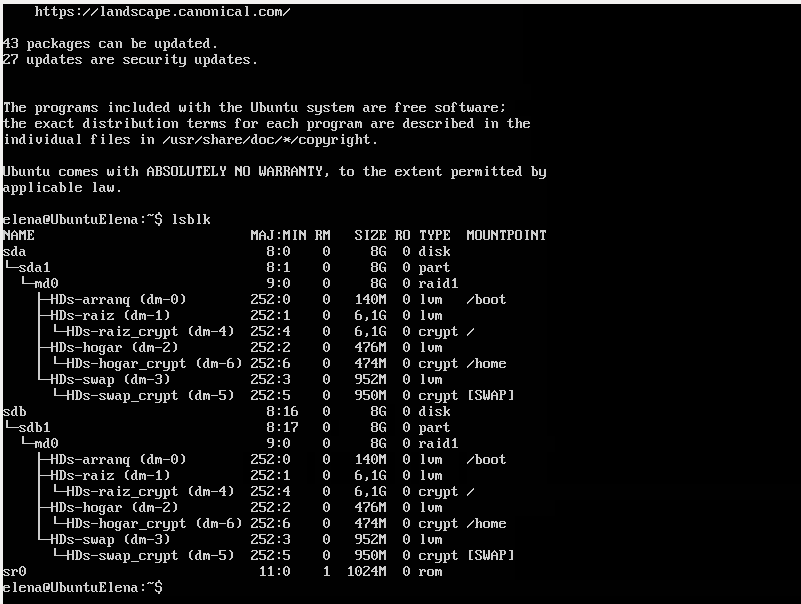
\includegraphics[scale=0.4]{img/P1-ubunturaidfunciona.png} 
\caption{Captura de pantalla de Ubuntu Server con la salida del comando lsblk} \label{fig:figura1}
\end{figure}



%----------------------------------------------------------------------------------------
%  Cuestión 11
%----------------------------------------------------------------------------------------

\section{Cuestión 11:}
\subsection{a) ¿Cómo ha hecho el disco 2 “arrancable”?}
Una vez iniciado sesión en Ubuntu Server instalo el grub en el disco 2 con el comando : grub-install /dev/sdb

\subsection{b) ¿Qué hace el comando grub-install?}
Instala el grub en el disco indicado como parámetro. El grub es un sistema gestor de arranque, mediante la selección de una
partición /boot.


%----------------------------------------------------------------------------------------
%  Cuestión opcional 1
%----------------------------------------------------------------------------------------

\section{Cuestión Opcional 1: Muestre (con capturas de pantalla) cómo ha comprobado que el RAID1 funciona.}
Para comprobar que funciona el RAID1 sobre Ubuntu Server, extraemos un disco del sistema y arrancamos el sistema.
Una vez iniciado el sistema sin problemas realizamos un lsblk para ver el estado de los discos, como se ve en la captura de pantalla \ref{fig:figura2}.
Si el RAID1 no funcionase no sería posible arrancar el sistema.
\begin{figure}[H] %con el [H] le obligamos a situar aquí la figura
\centering
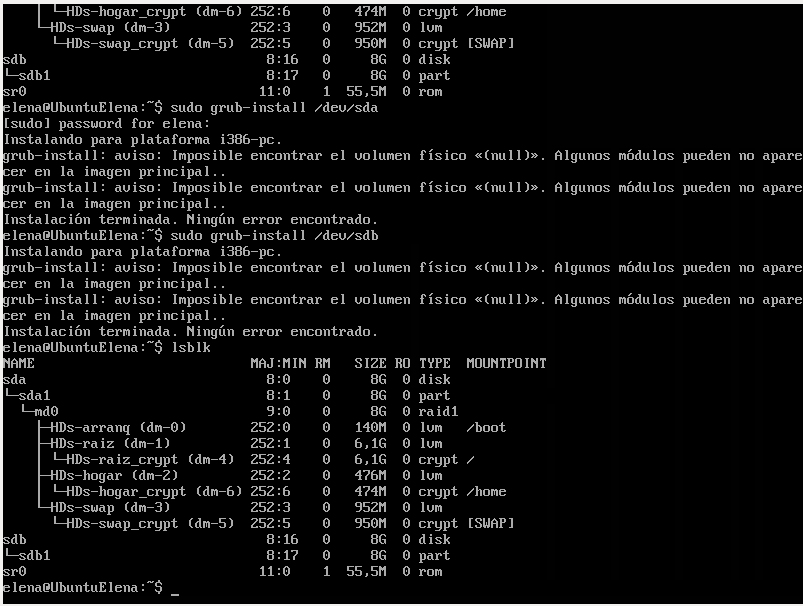
\includegraphics[scale=0.4]{img/P1-ubuntu-despuesdearrancarSinDisco.png} 
\caption{Captura de pantalla de Ubuntu Server con la salida del comando lsblk, despues de extraer un disco duro.} \label{fig:figura2}
\end{figure}

Ahora apagamos el sistema y volvemos a insertar el disco eliminado. Una vez arrancado el sistema sin problemas, tenemos que indicar al RAID1
que vamos a añadirle el nuevo disco, aunque ya este configurado, ya que el gestor del RAID1 tendrá un hueco disponible.
Esta operación se muestra en la captura de pantalla \ref{fig:figura3} y además se muestra el estado de los discos después.
\begin{figure}[H] %con el [H] le obligamos a situar aquí la figura
\centering
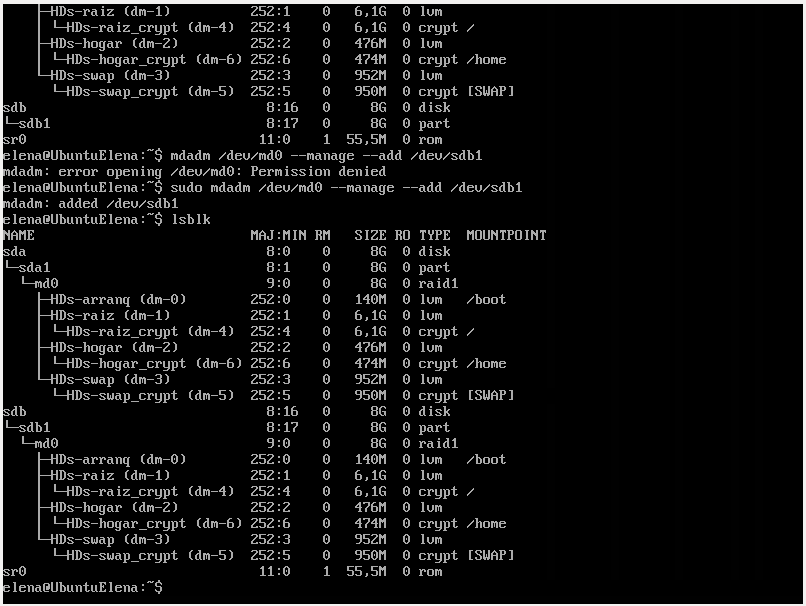
\includegraphics[scale=0.4]{img/ubuntuAnadidodenuevodiscoraid.png} 
\caption{Captura de pantalla de Ubuntu Server añadiendo disco al RAID1 y la salida del comando lsblk} \label{fig:figura3}
\end{figure}


%----------------------------------------------------------------------------------------
%  Cuestión 12
%----------------------------------------------------------------------------------------

\section{Cuestión 12 ¿Qué diferencia hay entre Standard y Datacenter?}
Según Microsoft \cite{Standar_DataCenter} \cite{Standar_DataCenter1}  cada versión va orientada a un público específico.\\
\textit{``La Standar va dirigida a servidores de baja densidad y entornos no virtualizados.''} \\
\textit{``La DataCenter va dirigida a servidores con alta virtualización y software de centro de datos.''}\\
En concreto la versión ``DataCenter'' es una versión muy superior en cuanto a prestaciones, ya que esta pensada para grandes servidores
de procesamiento de datos y estos requieren mayores prestaciones y equipos más potentes.




%----------------------------------------------------------------------------------------
%  Cuestión 13
%----------------------------------------------------------------------------------------

\section{Cuestión 13: Continúe usted con el proceso de definición de RAID1 para los dos discos de 50MiB que ha creado. Muestre el proceso con capturas de pantalla.}

Como se ve en la imagen \ref{fig:P1_E13_1} tenemos el disco 1 y disco 3 de 50Mib en la maquina virtual.

\begin{figure}[H] %con el [H] le obligamos a situar aquí la figura
\centering
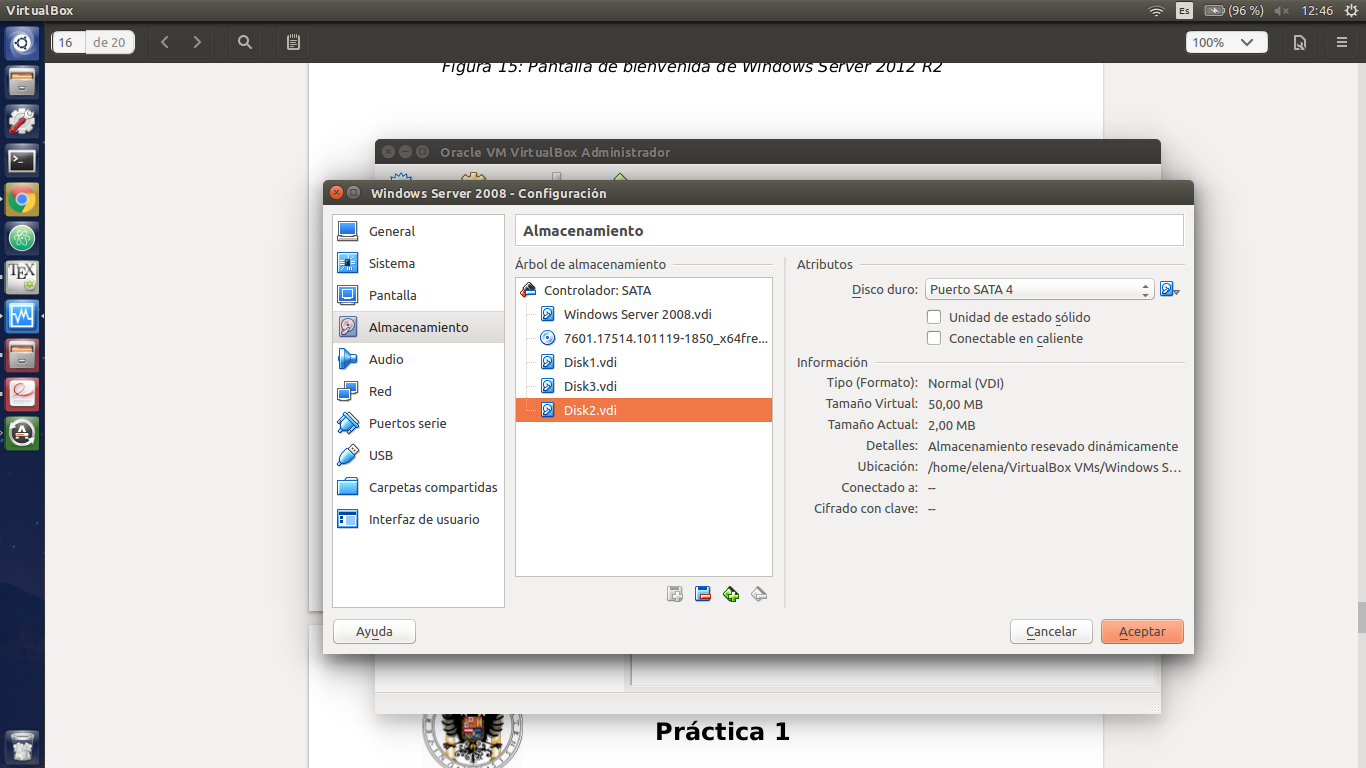
\includegraphics[scale=0.3]{img/P1-ejercicio13-1.png} 
\caption{Discos duros de Windows Server} \label{fig:P1_E13_1}
\end{figure}

Iniciamos Windows Server y vamos al Administrador de discos de Windows\ref{fig:P1_E13_2}.

\begin{figure}[H] %con el [H] le obligamos a situar aquí la figura
\centering
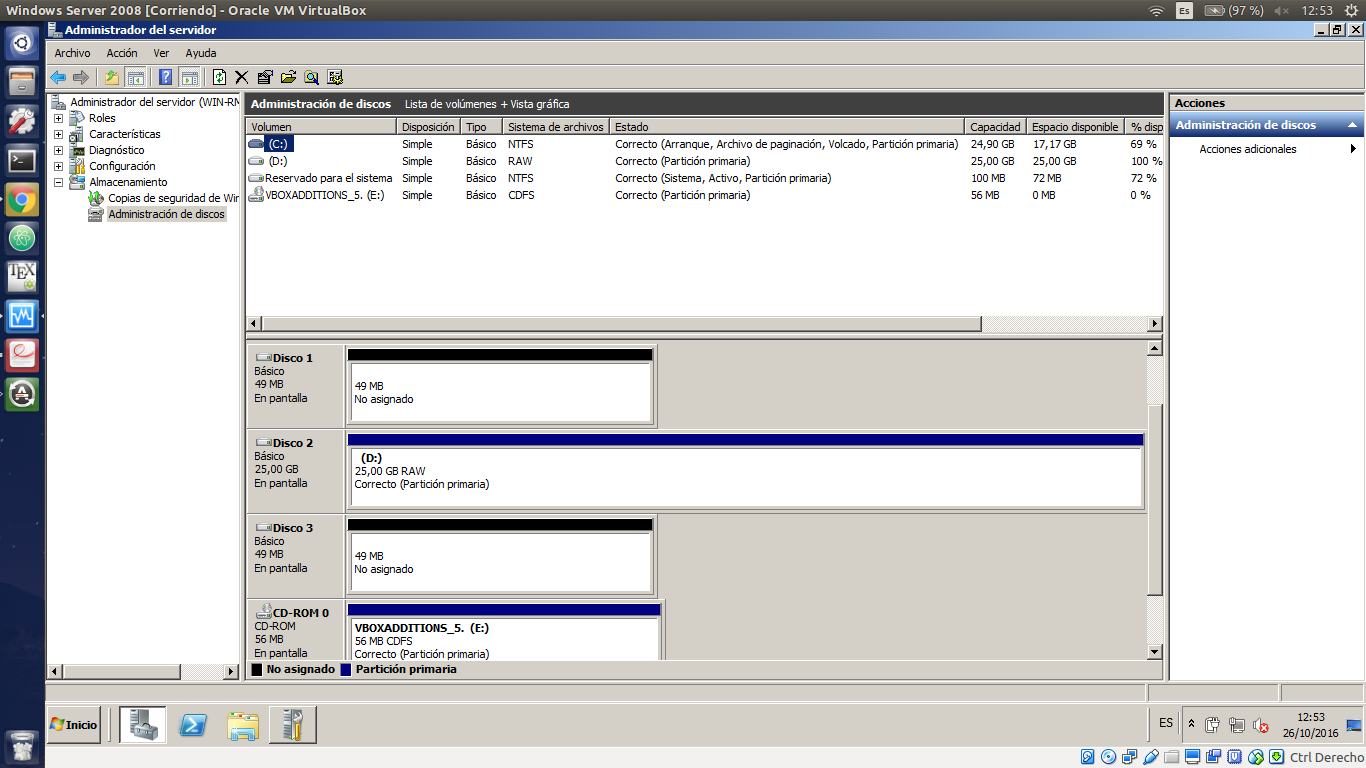
\includegraphics[scale=0.3]{img/P1-ejercicio13-2.png} 
\caption{Administrador de discos de Windows Server, antes del RAID} \label{fig:P1_E13_2}
\end{figure}

Para realizar el RAID, seleccionamos uno de los discos que pertenecerá al RAID y con ``Click'' derecho del ratón
seleccionamos la opción ``Nuevo volumen reflejado...'' \ref{fig:P1_E13_3}

\begin{figure}[H] %con el [H] le obligamos a situar aquí la figura
\centering
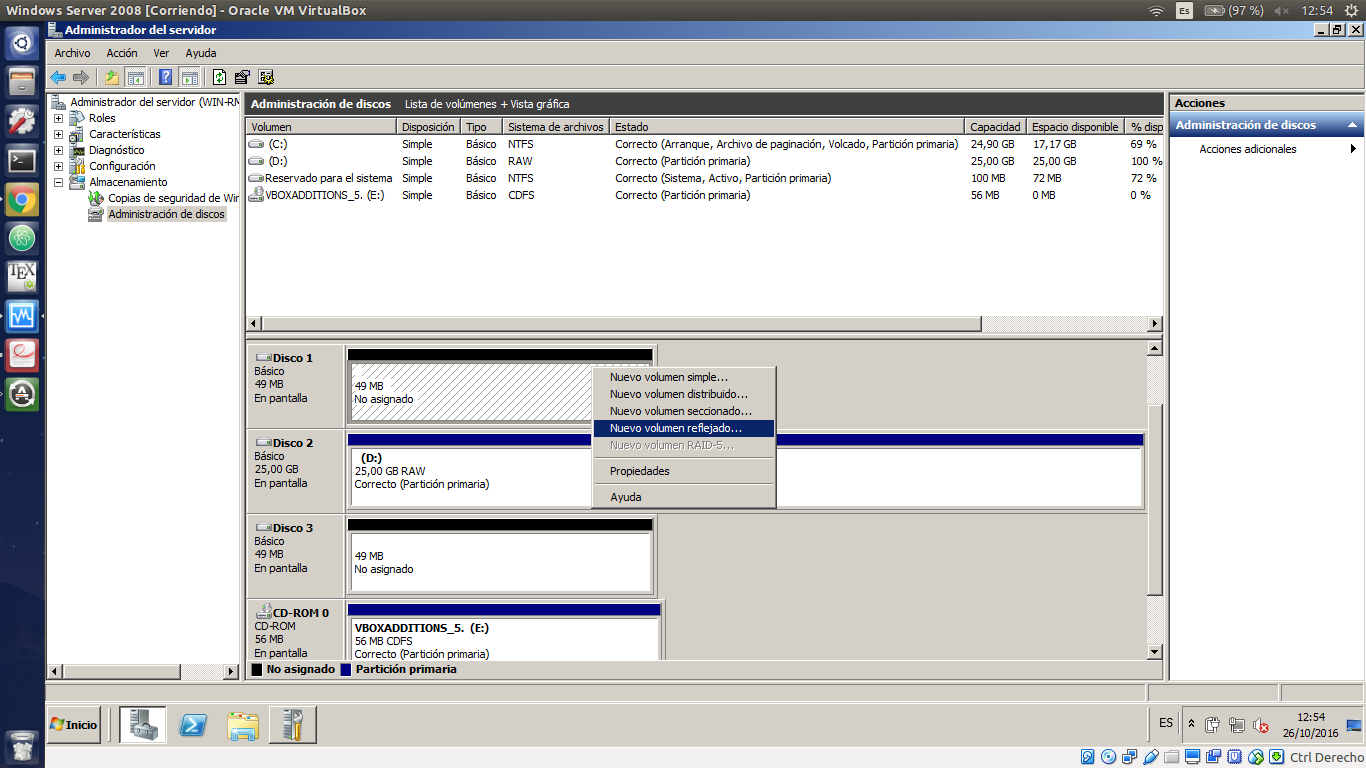
\includegraphics[scale=0.3]{img/P1-Ejercicio13-3.png} 
\caption{Administrador de discos de Windows Server, seleccionando disco duro para RAID} \label{fig:P1_E13_3}
\end{figure}

Una vez seleccionada la opción anterior nos saldrá el asistente de configuración de discos reflejados (RAID).
Avanzamos hasta que nos pregunte que discos pertenecerán al RAID \ref{fig:P1_E13_4}.

\begin{figure}[H] %con el [H] le obligamos a situar aquí la figura
\centering
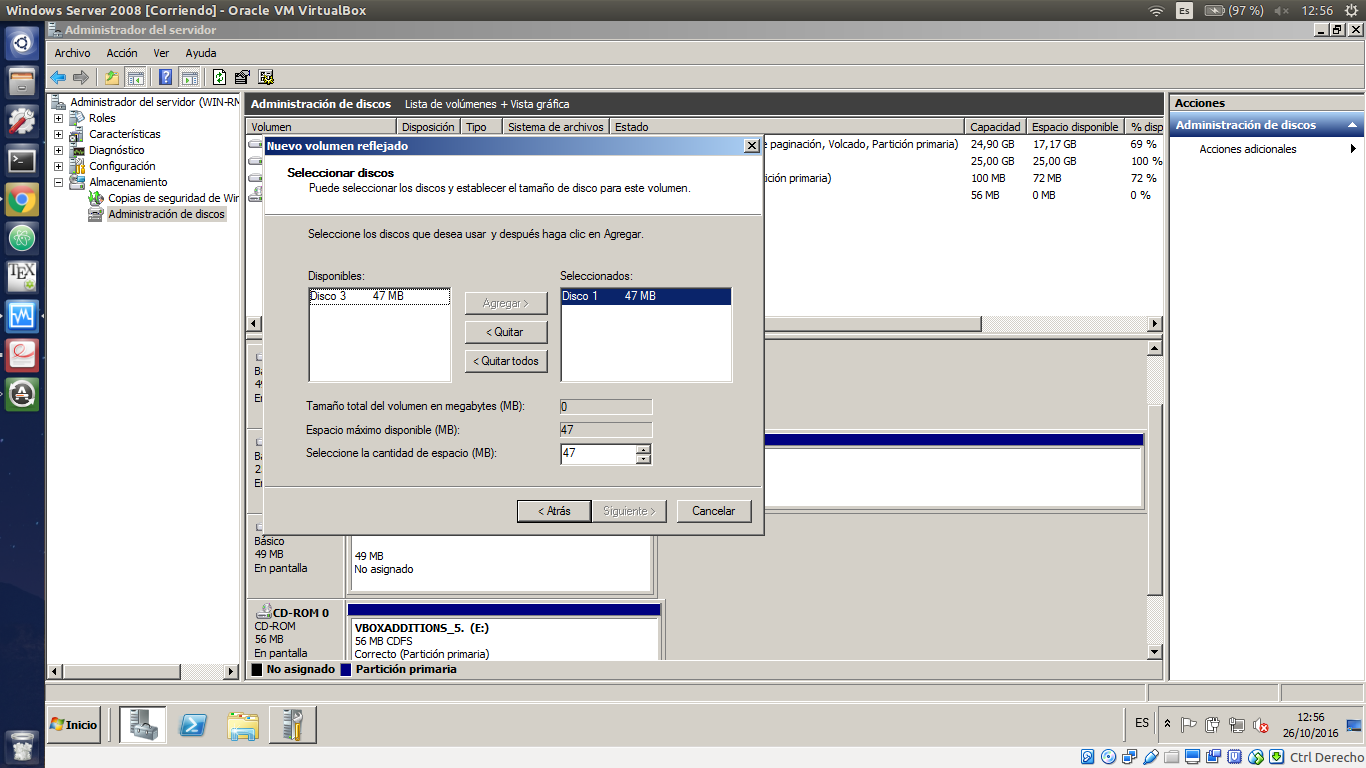
\includegraphics[scale=0.3]{img/P1-Ejercicio13-4.png} 
\caption{Asistente de Windows para crear RAID, selección de discos pertenecientes al raid} \label{fig:P1_E13_4}
\end{figure}

Añadimos los discos deseados, en nuestro caso el disco 1 y 3 \ref{fig:P1_E13_5}.

\begin{figure}[H] %con el [H] le obligamos a situar aquí la figura
\centering
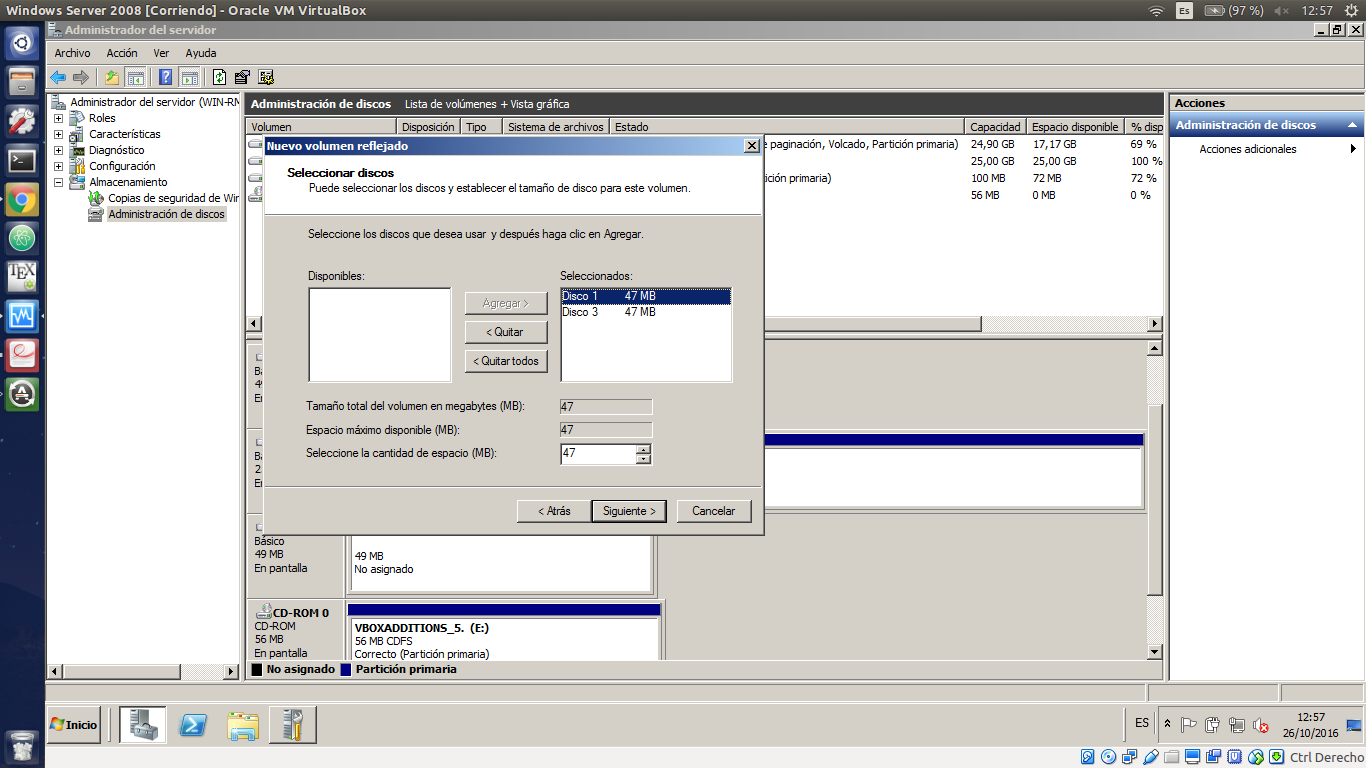
\includegraphics[scale=0.3]{img/P1-Ejercicio13-5.png} 
\caption{Asistente de Windows para crear RAID, discos pertenecientes al raid} \label{fig:P1_E13_5}
\end{figure}

Pasamos a los siguientes pasos, donde nos preguntará el punto de montaje\ref{fig:P1_E13_6} del RAID y el nombre del mismo.
Yo le he puesto mi nombre para identificar las capturas de pantalla como se puede observar en la captura \ref{fig:P1_E13_7}.
Finalizamos la configuración y observaremos que ahora en el Administrador de discos aparecen el disco 1 y 3 de color rosado, 
este color indica que es un RAID, como se ve en la captura \ref{fig:P1_E13_9}

\begin{figure}[H] %con el [H] le obligamos a situar aquí la figura
\centering
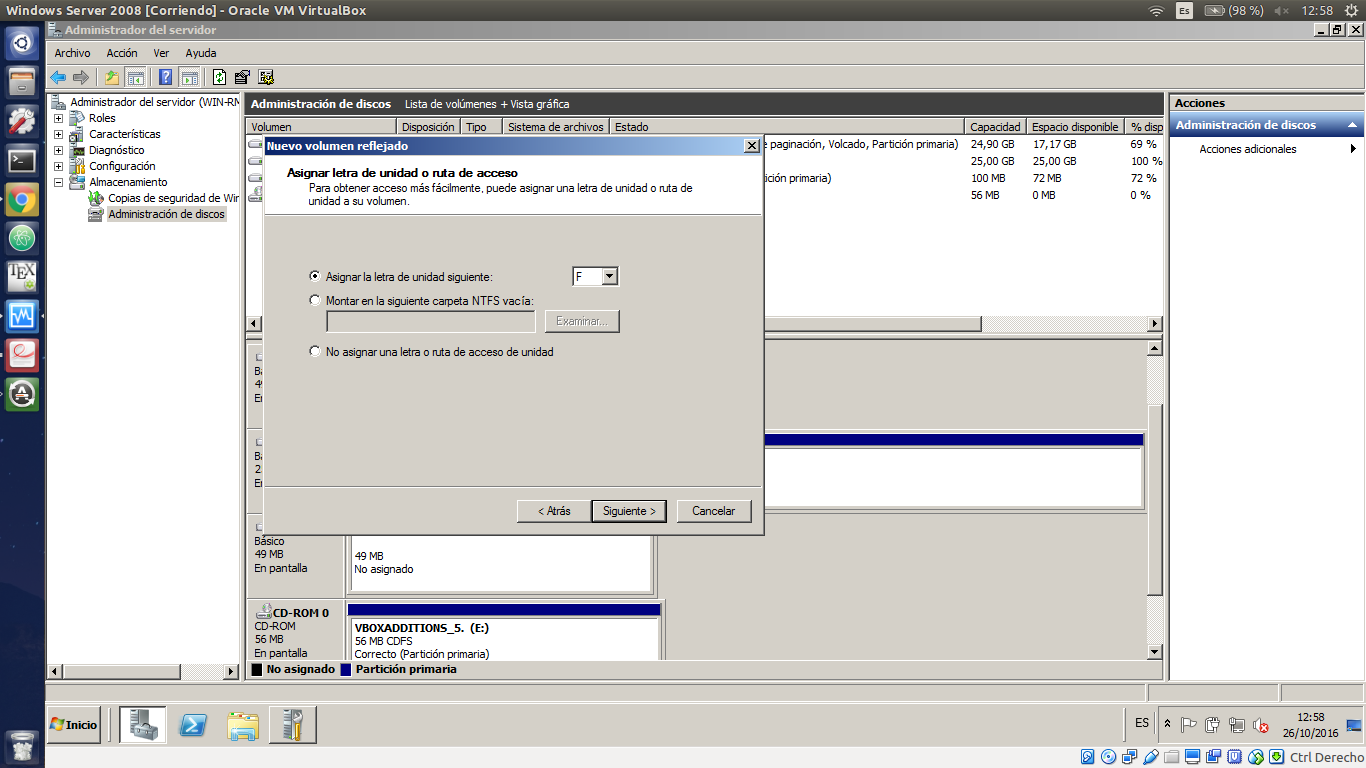
\includegraphics[scale=0.3]{img/P1-Ejercicio13-6.png} 
\caption{Asistente de Windows para crear RAID, punto de montaje del RAID} \label{fig:P1_E13_6}
\end{figure}

\begin{figure}[H] %con el [H] le obligamos a situar aquí la figura
\centering
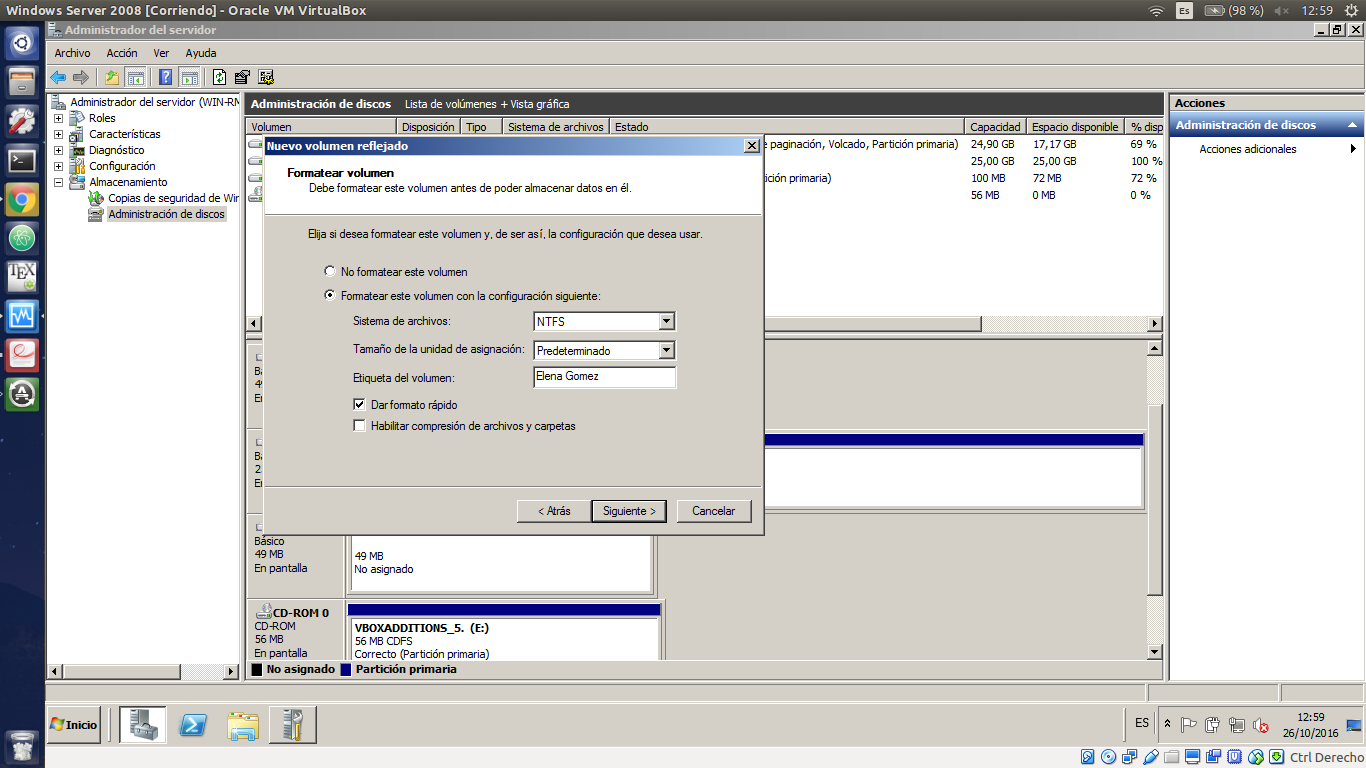
\includegraphics[scale=0.3]{img/P1-Ejercicio13-7.png} 
\caption{Asistente de Windows para crear RAID, información del RAID} \label{fig:P1_E13_7}
\end{figure}


\begin{figure}[H] %con el [H] le obligamos a situar aquí la figura
\centering
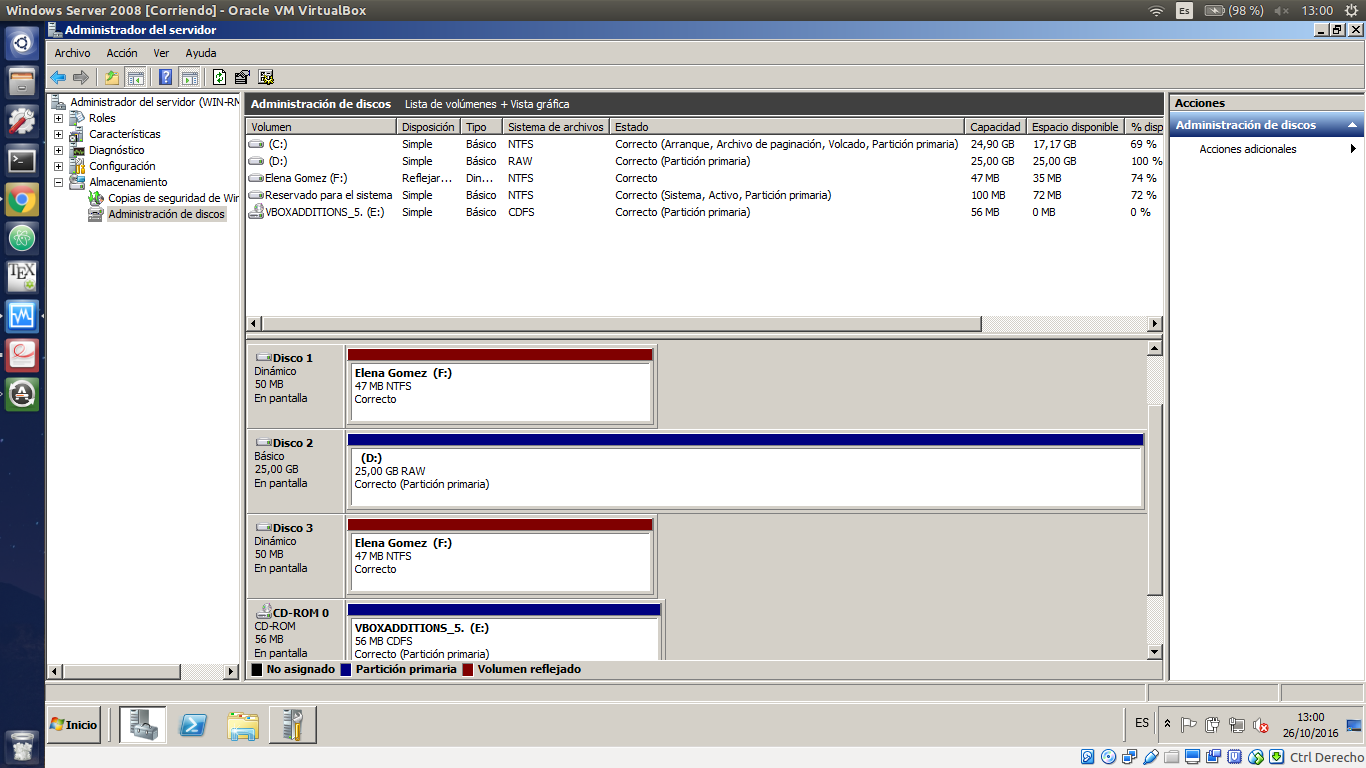
\includegraphics[scale=0.3]{img/P1-Ejercicio13-9.png} 
\caption{Administrador de discos de Windows Server, despues del RAID} \label{fig:P1_E13_9}
\end{figure}




%----------------------------------------------------------------------------------------
%  Cuestión 14
%----------------------------------------------------------------------------------------

\section{Cuestión 14: Explique brevemente qué diferencias hay entre los tres tipos
de conexión que permite el VMSW para las Mvs: NAT, Host-only y Bridge.}
Para VirtualBox \cite{VirtualBoxRedes} la diferencia de estos tipos de redes son:

En la red NAT es el VMSW el que realiza la función del router para el Sistema Operativo instalado en la máquina virtual.

En Host-only utiliza una red que contiene al anfitrión y a las máquinas virtuales sin necesidad de la interfaz de red del sistema anfitrión.

En Bridge es un tipo más avanzado para la simulación de servidores en las máquinas virtuales.





%------------------------------------------------

\bibliography{citas} %archivo citas.bib que contiene las entradas 
\bibliographystyle{plain} % hay varias formas de citar

\end{document}
